%Example of a few features of the accessibility package to make an accessible PDF document with tags, structure, and alt text.
\documentclass{article}
\usepackage[utf8]{inputenc}
\usepackage{graphicx}

%This package adds tags, structure, and alt text
%documentation and how-to can be found at https://ctan.org/pkg/accessibility
\usepackage[tagged, highstructure]{accessibility}

%This package allows equations/math to be readable
%documentation and how-to can be found at https://ctan.org/pkg/axessibility
\usepackage[accsupp]{axessibility}

\title{Example with Accessible and Axessible LaTeX packages}
\date{February 2023}

\begin{document}
\maketitle

\section{Introduction}
Some stuff here. Very exciting stuff!

\section{Skymap}
Figure \ref{fig:skymap} shows a fake skymap, created by generating Gaussian distributed x-y data:
\begin{equation}
    f(x) = \frac{1}{\sqrt{2 \pi \sigma^2}}e^{-\frac{1}{2}(\frac{x-\mu}{\sigma})^2}
\end{equation}
With $\sigma$ the standard deviation and $\mu=0$ the mean.

\begin{figure}
    \centering
    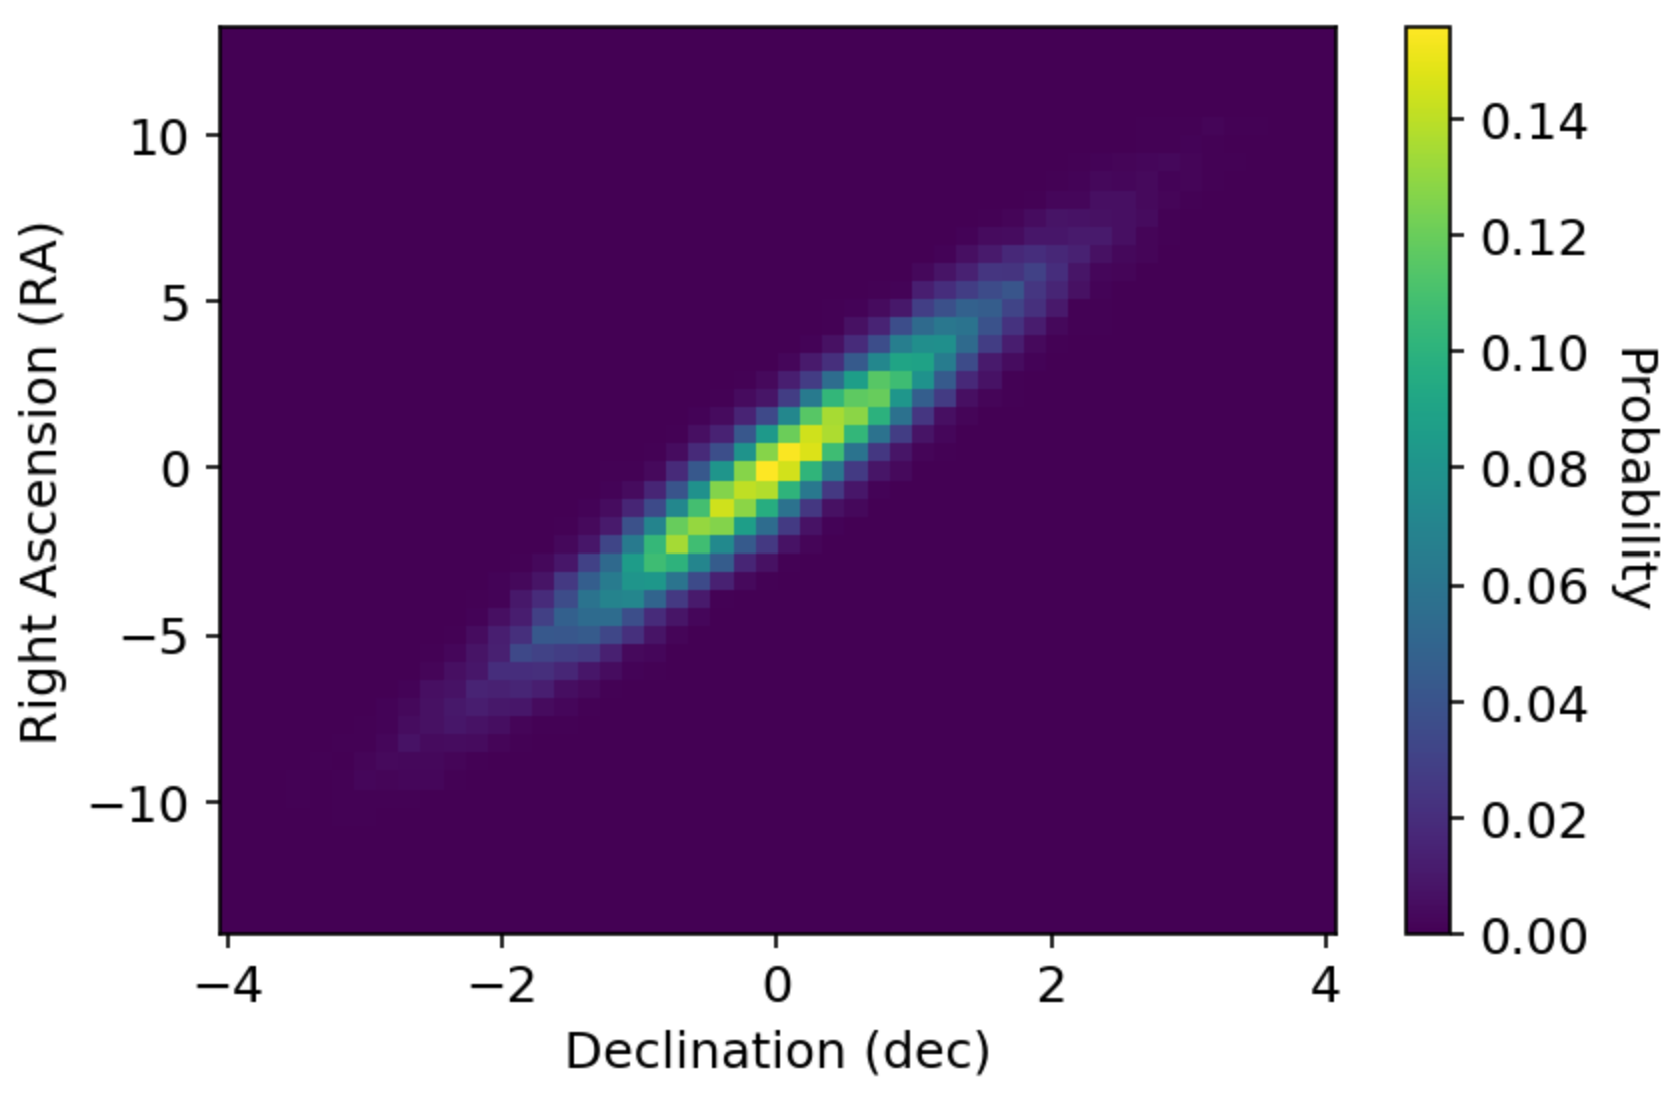
\includegraphics[width=\textwidth]{ex_map.png}
    \alt{2D histogram probability map of location of a potential source in right ascension and declination, where the highest probability region is centered around 0 degrees RA and dec and the spread in both RA and dec is Gaussian distributed.}
    \caption{Skymap showing the probability of a fake source location on the sky.}
    \label{fig:skymap}
\end{figure}

\end{document}
